\chapter{Introduction to more GSI Applications}\label{gsi_global}
\setlength{\parskip}{12pt}

%-------------------------------------------------------------------------------
\section{Introduction to Global GSI analysis}
%-------------------------------------------------------------------------------

The \textit{Global Forecast System (GFS)} is a global numerical weather prediction system containing a global computer model and variational analysis 
run by the U.S. National Weather Service (NWS). As of February 2015, the numerical model is run four times a day, and produces forecasts for up 
to 16 days in advance, with decreased spatial resolution after 10 days. It is a spectral model with a resolution of T1534 from 0 to 240 hours 
(0-10 days) and T574 from 240 to 384 hours (10-16 days). In the vertical, the model is divided into 64 layers and temporally, it produces forecast output 
every hour for the first 12 hours, every 3 hours out to 10 days, and every 12 hours after that. Its data assimilation system runs 6-hourly continuous cycles 
using the GSI-hybrid.

GSI has many functions specifically designed and tuned for GFS. Although the release version of the community GSI includes all the functions used by the 
operational systems, the DTC can only support the GSI regional applications because the DTC is not able to run GFS on community computers. Beginning 
with release version 3.2, the DTC began to introduce the use of GSI for global applications, assuming users can obtain the GFS background through the 
NCEP data hub or by running GFS themselves.

%-------------------------------------------------------------------------------
\subsection{The Difference between Global and Regional GSI}
%-------------------------------------------------------------------------------

As mentioned above, all of the NCEP operational systems use GSI as their analysis system. The majority of the GSI code is common to these 
operational systems. Very little source code is specific to a particular operational system. The main differences in the GSI operational application 
come from the configuration the run scripts and namelist parameters.

The different GSI applications need different backgrounds, observations, and fixed files. For the GFS system, GSI needs:

\begin{itemize}
\item GFS Backgrounds: Typically, GSI uses 6-h GFS forecasts as the background. GFS 3-h and 9-h forecasts are also needed for the FGAT function in 
the GSI analysis. Both surface and atmosphere forecasts are needed.
\item Observations: NCEP has several sets of BUFR/prepBUFR observation files with global coverage for global systems. The files that start with the 
prefix \textbf{GDAS} are for the 6-hourly global data assimilation system. These files have more data available for the analysis, but have a longer delay 
for use in real-time. The files that start with \textbf{gfs} are for the GFS forecasts. Different operational systems need different observation data files because they require different kinds of observations with different coverage, cut-off times, and quality control processes. All these observation 
files are read in and processed in GSI by the same section of code. Therefore, there is no problem using GFS observation data files for regional GSI 
applications, as is described in the practice cases and the GSI User\textquotesingle s Guide. Using regional BUFR files for global applications will cause 
problems since the data only cover part of the analysis domain, but GSI can still read in the observations and perform the analysis.
\item Fixed files: Section 3.1 of the GSI User\textquotesingle s Guide introduced the notion that different operational systems have their own fixed files. 
These global fixed files can be downloaded as a separate tar ball from the GSI user\textquotesingle s website 
(\url{http://www.dtcenter.org/com-GSI/users/downloads/index.php}). For the GFS GSI application, the big difference is the background error covariance (BE). 
Different resolutions of the GFS backgrounds use their matched BE files, which are different from the BE files used by the regional GSI applications. In 
release version 3.4, ten new BE files were provided for users (in addition to the two for release version 3.3): \\
\begin{enumerate}
\item \verb| global_berror.l64y386.f77  |
\item \verb| global_berror.l64y96.f77  |
\item \verb| global_berror.l64y1154.f77 |	
\item \verb| global_berror.l64y290.f77 |	
\item \verb| global_berror.l64y882.f77 |
\item \verb| global_berror.l64y130.f77 |		
\item \verb| global_berror.l64y192.f77 |	
\item \verb| global_berror.l64y578.f77 |
\item \verb| global_berror.l64y258.f77 |	
\item \verb| global_berror.l64y674.f77 |
\end{enumerate}
\end{itemize}

%-------------------------------------------------------------------------------
\subsection{Global GFS Scripts}
%-------------------------------------------------------------------------------

Starting with release version 3.3, support for running GSI global applications was added to the community release. Specifically a sample global analysis 
run script was added to the \verb|./run| directory named \verb|run_gsi_global.ksh| of the community release. This script \verb|run_gsi_global.ksh| is 
based on the GSI GFS regression tests. This script retains the same basic structure as the regional run script \verb|run_gsi_regional.ksh|, but includes 
additional details needed for the global analysis. 

\begin{table}[htbp]
\centering
\caption{The grid dimensions for GFS.}
\begin{tabular}{|p{3cm}|p{4.5cm}|p{4.45cm}|}
\hline
&EULERIAN&SEMI-LAGRANGIAN\\
\end{tabular}
\begin{tabular}{|p{3cm}|p{2cm}|p{2cm}|p{2cm}|p{2cm}|}
\hline
SPECTRAL RESOLUTION &  LONB & LATB & LONB & LATB \\
\hline
T62&192&94&128&64\\
\hline
T126&384&190&256&128\\
\hline
T170&512&256&352&176\\
\hline
T190&576&288&384&192\\
\hline
T254&768&384&512&256\\
\hline
T382&1152&576&768&384\\
\hline
T574&1760&880&1152&576\\
\hline
T878&2304&1152&1760&880\\
\hline
T1148&&&2304&1152\\
\hline
T1534&&&3072&1536\\
\hline
T2014&&&4032&2016\\
\hline
T2046&&&4096&2048\\
\hline
T3070&&&6144&3072\\
\hline
\end{tabular}
\label{ch6_table1}
\end{table} 

The first part of the global analysis run script, just as in the regional script, sets up the computer environment and case configuration. The primary 
differences between the global and regional scripts are the specification of the GFS case and the global application namelist.
\begin{small}
\begin{verbatim}
     GFSCASE=T126
     GSI_NAMELIST=${GSI_ROOT}/run/comgsi_namelist_gfs.sh
\end{verbatim}
\end{small}
While the regional script simply specifies the background and BE files, the global script needs to know the background resolution by defining the 
following parameters:
\begin{scriptsize}
\begin{verbatim}
# Set the JCAP resolution which you want.
# All resolutions use LEVS=64
if [[ "$GFSCASE" = "T62" ]]; then
  JCAP=62
  JCAP_B=62
elif [[ "$GFSCASE" = "T126" ]]; then
  JCAP=126
  JCAP_B=126
elif [[ "$GFSCASE" = "enkf_glb_t254" ]]; then
  JCAP=254
  JCAP_B=254
elif [[ "$GFSCASE" = "T254" ]]; then
  JCAP=254
  JCAP_B=574
elif [[ "$GFSCASE" = "T574" ]]; then
  JCAP=574
  JCAP_B=1534
else
   echo "INVALID case = $GFSCASE"
   exit
fi
  LEVS=64
#
\end{verbatim}
\end{scriptsize}

Just as with the regional analysis run script, the global script double checks the needed parameters, creates a run directory, and copies the background, observations, and fixed files into the run directory. It generates the namelist, and places it in the run directory as well. 
\begin{enumerate}
\item Specify the values of \verb|LATA|, \verb|LONA|, \verb|DELTIME|, \verb|resol| based on the choice of \verb|JCAP|:
\begin{scriptsize}
\begin{verbatim}
# Given the requested resolution, set dependent resolution parameters
if [[ "$JCAP" = "382" ]]; then
   LONA=768
   LATA=384
   DELTIM=180
   resol=1
elif [[ "$JCAP" = "574" ]]; then
   LONA=1152
   LATA=576
   DELTIM=1200
   resol=2
elif [[ "$JCAP" = "254" ]]; then
   LONA=512
   LATA=256
   DELTIM=1200
   resol=2
elif [[ "$JCAP" = "126" ]]; then
   LONA=256
   LATA=128
   DELTIM=1200
   resol=2
elif [[ "$JCAP" = "62" ]]; then
   LONA=192
   LATA=94
   DELTIM=1200
   resol=2
else
   echo "INVALID JCAP = $JCAP"
   exit
fi
NLAT=` expr $LATA + 2 `
\end{verbatim}
\end{scriptsize}
\item Set up CO2, CH4, N2O, CO file decisions:
\begin{scriptsize}
\begin{verbatim}
ICO2=${ICO2:-0}
if [ $ICO2 -gt 0 ] ; then
        # Copy co2 files to $workdir
        co2dir=${FIX_ROOT}
        yyyy=`echo $ANAL_TIME | cut -c1-4`
        rm ./global_co2_data.txt
        co2=$co2dir/global_co2.gcmscl_$yyyy.txt
        while [ ! -s $co2 ] ; do
                ((yyyy-=1))
                co2=$co2dir/global_co2.gcmscl_$yyyy.txt
        done
        if [ -s $co2 ] ; then
                cp $co2 ./global_co2_data.txt
        fi
        if [ ! -s ./global_co2_data.txt ] ; then
                echo "\./global_co2_data.txt" not created
                exit 1
        fi
fi
#CH4 file decision
...

\end{verbatim}
\end{scriptsize}
\item Set up the namelist parameters and generate the namelist:
\begin{scriptsize}
\begin{verbatim}
# Set some parameters for use by the GSI executable and to build the namelist
echo " Build the namelist "

vs_op='0.7,'
hzscl_op='1.7,0.8,0.5,'

... ...

# Build the GSI namelist on-the-fly
. $GSI_NAMELIST
cat << EOF > gsiparm.anl

 $comgsi_namelist

EOF
\end{verbatim}
\end{scriptsize}
\item Multiple time level backgrounds are needed:
\begin{scriptsize}
\begin{verbatim}
if [[ "$GFSCASE" = "enkf_glb_t254" ]]; then
  cp $OBS_ROOT/gdas1.t12z.abias      ./satbias_in
  cp $OBS_ROOT/gdas1.t12z.satang     ./satbias_angle

  cp $BK_ROOT/sfcanl_2014040506_fhr03_ensmean  ./sfcf03
  cp $BK_ROOT/sfcanl_2014040506_fhr06_ensmean  ./sfcf06
  cp $BK_ROOT/sfcanl_2014040506_fhr06_ensmean  ./sfcf09

  cp $BK_ROOT/sfg_2014040506_fhr03_mem001    ./sigf03
  cp $BK_ROOT/sfg_2014040506_fhr06_mem001    ./sigf06
  cp $BK_ROOT/sfg_2014040506_fhr09_mem001    ./sigf09
else
  cp $OBS_ROOT/satbias_in            ./satbias_in
  cp $OBS_ROOT/satbias_angle         ./satbias_angle

  cp $BK_ROOT/sfcf03  ./sfcf03
  cp $BK_ROOT/sfcf06  ./sfcf06
  cp $BK_ROOT/sfcf09  ./sfcf09

  cp $BK_ROOT/sigf03  ./sigf03
  cp $BK_ROOT/sigf06  ./sigf06
  cp $BK_ROOT/sigf09  ./sigf09
fi
\end{verbatim}
\end{scriptsize}
Both surface and atmosphere files at 03, 06, and 09 hour forecasts are needed. \\
\item More observations files are available\\
In the sample run script, many more observations are listed for use:
\begin{scriptsize}
\begin{verbatim}
# Link to the other observation data

if [[ "$GFSCASE" = "enkf_glb_t254" ]]; then
  obsfile_amua=gdas1.t12z.1bamua.tm00.bufr_d
  obsfile_amub=gdas1.t12z.1bamub.tm00.bufr_d
else
  obsfile_amua=amsuabufr
  obsfile_amub=amsubbufr
fi

if [ -r "${OBS_ROOT}/satwnd" ]; then
   ln -s ${OBS_ROOT}/satwnd .
fi
if [ -r "${OBS_ROOT}/gpsrobufr" ]; then
   ln -s ${OBS_ROOT}/gpsrobufr .
fi

......

if [ -r "${OBS_ROOT}/amsubbufrears" ]; then
   ln -s ${OBS_ROOT}/amsubbufrears .
fi
if [ -r "${OBS_ROOT}/tcvitl" ]; then
   ln -s ${OBS_ROOT}/tcvitl .
fi
\end{verbatim}
\end{scriptsize}
\end{enumerate}

Table \ref{ch6_table1} lists the grid dimensions for GFS of different resolutions from \textit{Running Global Model Parallel Experiments Version 6.0} from NCEP/EMC, which may provide users more information on the above mentioned resolution parameters:


%-------------------------------------------------------------------------------
\subsection{Sample Results}
%-------------------------------------------------------------------------------

After a successful run of the GSI GFS analysis, the contents of the run directory, with the clean option turned on, will look something like this:
\begin{scriptsize}
\begin{verbatim}
amsrebufr                              diag_mhs_n18_anl.2011080100.gz       fort.213
amsuabufr                              diag_mhs_n18_ges.2011080100.gz       fort.214
amsubbufr                              diag_mhs_n19_anl.2011080100.gz       fort.215
anavinfo                               diag_mhs_n19_ges.2011080100.gz       fort.217
atms_beamwidth.txt                     diag_omi_aura_anl.2011080100.gz      fort.218
berror_stats                           diag_omi_aura_ges.2011080100.gz      fort.219
bftab_sstphr                           diag_pcp_tmi_trmm_anl.2011080100.gz  fort.220
convinfo                               diag_pcp_tmi_trmm_ges.2011080100.gz  fort.221
diag_amsre_hig_aqua_anl.2011080100.gz  diag_sbuv2_n16_anl.2011080100.gz     gomebufr
diag_amsre_hig_aqua_ges.2011080100.gz  diag_sbuv2_n16_ges.2011080100.gz     gpsrobufr
diag_amsre_low_aqua_anl.2011080100.gz  diag_sbuv2_n17_anl.2011080100.gz     gsi.exe
diag_amsre_low_aqua_ges.2011080100.gz  diag_sbuv2_n17_ges.2011080100.gz     gsiparm.anl
diag_amsre_mid_aqua_anl.2011080100.gz  diag_sbuv2_n18_anl.2011080100.gz     hirs3bufr
diag_amsre_mid_aqua_ges.2011080100.gz  diag_sbuv2_n18_ges.2011080100.gz     hirs4bufr
diag_amsua_metop-a_anl.2011080100.gz   diag_sbuv2_n19_anl.2011080100.gz     mhsbufr
diag_amsua_metop-a_ges.2011080100.gz   diag_sbuv2_n19_ges.2011080100.gz     omibufr
diag_amsua_n15_anl.2011080100.gz       diag_seviri_m09_anl.2011080100.gz    ozinfo
diag_amsua_n15_ges.2011080100.gz       diag_seviri_m09_ges.2011080100.gz    pcpbias_out
diag_amsua_n18_anl.2011080100.gz       errtable                             pcpinfo
diag_amsua_n18_ges.2011080100.gz       fit_p1.2011080100                    prepbufr
diag_amsua_n19_anl.2011080100.gz       fit_q1.2011080100                    prepobs_prep.bufrtable
diag_amsua_n19_ges.2011080100.gz       fit_rad1.2011080100                  satbias_angle
diag_amsub_n17_anl.2011080100.gz       fit_t1.2011080100                    satbias_in
diag_amsub_n17_ges.2011080100.gz       fit_w1.2011080100                    satbias_out
diag_conv_anl.2011080100.gz            fort.201                             satinfo
diag_conv_ges.2011080100.gz            fort.202                             satwnd
diag_gome_metop-a_anl.2011080100.gz    fort.203                             sbuvbufr
diag_gome_metop-a_ges.2011080100.gz    fort.204                             scaninfo
diag_hirs3_n17_anl.2011080100.gz       fort.205                             seviribufr
diag_hirs3_n17_ges.2011080100.gz       fort.206                             sfcanl.gsi
diag_hirs4_metop-a_anl.2011080100.gz   fort.207                             siganl
diag_hirs4_metop-a_ges.2011080100.gz   fort.208                             stdout
diag_hirs4_n19_anl.2011080100.gz       fort.209                             stdout.anl.2011080100
diag_hirs4_n19_ges.2011080100.gz       fort.210                             tcvitl
diag_mhs_metop-a_anl.2011080100.gz     fort.211                             tmirrbufr
diag_mhs_metop-a_ges.2011080100.gz     fort.212
\end{verbatim}
\end{scriptsize}

The majority of these files existed after running the GSI regional analysis examples in section \ref{sec3.2.3} of the Basic User\textquotesingle s 
Guide, and they provide the same information about the GSI run. Of note, the GSI global analysis run includes more radiance observations, resulting 
in more radiance \verb|diag| files in this list. Instead of the single background file \verb|wrf_inout| as seen with the regional analysis, the global analysis background is split between the two files \verb|siganl|, for the atmosphere, and \verb|sfcanl.gsi| for the surface. A quick check of the standard output file 
\verb|stdout| shows information similar to that generated by the regional runs for the namelist, data ingest, and minimization, but is quite different with respect to information on the background IO.

Please visit our online tutorial for more details regarding how to conduct a global GSI run.

%-------------------------------------------------------------------------------
\section{Introduction to Chemical Analysis}
%-------------------------------------------------------------------------------

The GSI has also been developed to analyze chemical observations, such as MODIS AOD or PM2.5, to improve the pollution forecasts with chemical models. 
In this release, GSI can do the following chemical analyses:

\begin{table}[htbp]
\centering
\caption{List of GSI chemical analyses}
\begin{tabular}{|p{1cm}|p{3cm}|p{4cm}|p{3cm}|}
\hline
case&Chemical Model &background species & Observations\\
\hline
1&WRF-Chem &  GOCART & MODIS AOD \\
\hline
2&WRF-Chem &  GOCART & PM2.5 \\
\hline
3&WRF-Chem &  PM2.5 & PM2.5 \\
\hline
4&CMAQ &  CMAQ & PM2.5 \\
\hline
\end{tabular}
\label{tab62}
\end{table} 

The GSI run script for a chemical analysis (\verb|./run/run_gsi_chem.ksh| ) and associated namelist (\verb|./run/comgsi_namelist_chem.sh|) are provided with this release. 
Sample background and observation files are provided through the on-line tutorial. 

%-------------------------------------------------------------------------------
\subsection{Setup GSI Run Scripts for Chemical Analysis}
%-------------------------------------------------------------------------------

The script \verb|run_gsi_chem.ksh| was built based on regional GSI run scripts and has a similar structure to the regional run script \verb|run_gsi_regional.ksh|, 
but include a couple of differences.

The first part of the run script sets up the computer environment and case configuration. This is similar to the regional analysis run scripts, except 
for the specification of (\verb|bk_core| and \verb|obs_type|) for a given chemical case, and the namelist for the chemical application:
\begin{scriptsize}
\begin{verbatim}
GSI_NAMELIST=${GSI_ROOT}/run/comgsi_namelist_chem.sh

#------------------------------------------------
# bk_core= set background (WRFCHEM_GOCART WRFCHEM_PM25 or CMAQ)
# obs_type= set observation type (MODISAOD or PM25)
  bk_core=CMAQ
  obs_type=PM25
\end{verbatim}
\end{scriptsize}
The choices of (\verb|bk_core| and \verb|obs_type|) for a chemical case need to match with the options \verb|PREPBUFR| and \verb|BK_FILE|, which set background and observation files. Table \ref{tab63} shows how to set up these two options for each case:

\begin{table}[htbp]
\centering
\begin{footnotesize}
\caption{List of GSI chemical analyses.}
\begin{tabular}{|p{0.7cm}|p{7cm}|p{7cm}|}
\hline
case&background (\textit{BK\_FILE} ; \textit{bk\_core} ) & Observation (\textit{PREPBUFR}; \textit{obs\_type})\\
\hline
1&wrfinput\_enkf\_d01\_2012-06-03\_18:00:00;  & Aqua\_Terra\_AOD\_BUFR:2012-06-03\_00:00:00;  \\
&WRFCHEM\_GOCART &  MODISAOD \\
\hline
2&wrfinput\_enkf\_d01\_2012-06-03\_18:00:00;  & anow.2012060318.bufr; \\
 & WRFCHEM\_GOCART &  PM25\\
\hline
3&wrfinput\_enkf\_d01\_2012-06-03\_18:00:00; & anow.2012060318.bufr; \\
& WRFCHEM\_PM25&  PM25 \\
\hline
4&cmaq2gsi\_4.7\_20130621\_120000.bin;  & anow.2013062112.bufr; \\
& CMAQ & PM25\\
\hline
\end{tabular}
\label{tab63}
\end{footnotesize}
\end{table} 
Similar to the regional run script, this chemical run script will also double check the needed parameters. Then it creates a run directory, generates the namelist, and copies the background, observations, and fixed files into the run directory. Users who run the cases listed in table \ref{tab62} do not need to change the rest of the run script. But users who need to build new cases may need to know the differences between chemical and regional applications, which is shown below.  

\begin{enumerate}
\item Specify the name of the background and observations:
\begin{scriptsize}
\begin{verbatim}
# Bring over background field (it's modified by GSI so we can't link to it)

if [ ${bk_core} = WRFCHEM_GOCART ] ; then
   cp ${BK_FILE} ./wrf_inout
fi
if [ ${bk_core} = WRFCHEM_PM25 ] ; then
   cp ${BK_FILE} ./wrf_inout
fi
if [ ${bk_core} = CMAQ ] ; then
   cp ${BK_FILE} ./cmaq_in.bin
fi

# Link to the observation data
if [ ${obs_type} = MODISAOD ] ; then
 ln -s ${PREPBUFR} ./modisbufr
fi
if [ ${obs_type} = PM25 ] ; then
 ln -s ${PREPBUFR} ./pm25bufr
fi
\end{verbatim}
\end{scriptsize}
\item Specify the background error file and anavinfo:
\begin{scriptsize}
\begin{verbatim}
if [ ${bk_core} = WRFCHEM_GOCART ] ; then
  BERROR=${FIX_ROOT}/wrf_chem_berror_little_endian
  BERROR_CHEM=${FIX_ROOT}/wrf_chem_berror_little_endian
  ANAVINFO=${FIX_ROOT}/anavinfo_wrfchem_gocart
fi
if [ ${bk_core} = WRFCHEM_PM25 ] ; then
  BERROR=${FIX_ROOT}/wrf_chem_berror_little_endian
  BERROR_CHEM=${FIX_ROOT}/wrf_chem_berror_little_endian
  ANAVINFO=${FIX_ROOT}/anavinfo_wrfchem_pm25
fi
if [ ${bk_core} = CMAQ ] ; then
  BERROR=${FIX_ROOT}/cmaq_berror_little_endian
  BERROR_CHEM=${FIX_ROOT}/cmaq_berror_little_endian
  ANAVINFO=${FIX_ROOT}/anavinfo_cmaq_pm25
fi
\end{verbatim}
\end{scriptsize}
\item Specify the options for building the namelist:
\begin{scriptsize}
\begin{verbatim}
if [ ${bk_core} = WRFCHEM_GOCART ] ; then
 bk_core_arw='.true.'
 bk_if_netcdf='.true.'
 bk_core_cmaq='.false.'
 bk_wrf_pm2_5='.false.'
 bk_laeroana_gocart='.true.'
fi
if [ ${bk_core} = WRFCHEM_PM25 ] ; then
 bk_core_arw='.true.'
 bk_if_netcdf='.true.'
 bk_core_cmaq='.false.'
 bk_wrf_pm2_5='.true.'
 bk_laeroana_gocart='.false.'
fi
if [ ${bk_core} = CMAQ ] ; then
 bk_core_arw='.false.'
 bk_if_netcdf='.false.'
 bk_core_cmaq='.true.'
 bk_wrf_pm2_5='.false.'
 bk_laeroana_gocart='.false.'
fi
\end{verbatim}
\end{scriptsize}
\end{enumerate}

%-------------------------------------------------------------------------------
\subsection{Sample Results}
%-------------------------------------------------------------------------------

In this section, case one in Table \ref{tab62} will be used as an example. After a successful run of the GSI Chem analysis, the contents of the run directory, with the clean option turned on, will look something like this:
\begin{scriptsize}
\begin{verbatim}
aeroinfo                  fit_w1.2012060318  fort.212  fort.226            pcpinfo
anavinfo                  fort.201           fort.213  fort.227            prepobs_prep.bufrtable
berror_stats              fort.202           fort.214  fort.228            satbias_angle
berror_stats_chem         fort.203           fort.215  fort.229            satbias_in
convinfo                  fort.204           fort.217  fort.230            satbias_out
diag_conv_anl.2012060318  fort.205           fort.218  gsi.exe             satinfo
diag_conv_ges.2012060318  fort.206           fort.219  gsiparm.anl         stdout
errtable                  fort.207           fort.220  l2rwbufr            stdout.anl.2012060318
fit_p1.2012060318         fort.208           fort.221  list_run_directory  wrfanl.2012060318
fit_q1.2012060318         fort.209           fort.223  modisbufr           wrf_inout
fit_rad1.2012060318       fort.210           fort.224  ozinfo
fit_t1.2012060318         fort.211           fort.225  pcpbias_out
\end{verbatim}
\end{scriptsize}

Following instructions from Chapter 5, the following steps are conducted to check the results of this GSI chemical analysis:

\begin{enumerate}
\item Check the standard output file: \\

\begin{itemize}
\item Read in chemical background fields:
\begin{scriptsize}
\begin{verbatim}
  rmse_var=sulf
  ordering=XYZ
  WrfType,WRF_REAL=         104         104
  ndim1=           3
  staggering= N/A
  start_index=           1           1           1           0
  end_index=         112         122          40           0
  k,max,min,mid var=sulf                                      1   9.622933
  3.3167184E-13  0.7885093
  k,max,min,mid var=sulf                                      2   9.687045  
  3.3167214E-13  0.7910572
... ...
  rmse_var=BC1
  ...
  rmse_var=BC2
  ...
  rmse_var=OC1
  ...
  rmse_var=OC2
  ...

\end{verbatim}
\end{scriptsize}

\item Read in modis AOD observations:
\begin{tiny}
\begin{verbatim}
OBS_PARA: modis_aod terra              7        64        50        11        34        25         7        81
                  40        31        50        27        38        46        56        25         7         0
                  26        53        62        60        19         0
OBS_PARA: modis_aod aqua              29        34        44        23        50        18        55        76
                  33        30        49        22        20        67        76        30         2         0
                  36        76        38        50        14         0
\end{verbatim}
\end{tiny}

\item Minimizations:
\begin{scriptsize}
\begin{verbatim}
 Begin J table inner/outer loop           0           1
     J term                                     J
aerosol aod                  7.8897778549100276E+03
 -----------------------------------------------------
J Global                    7.8897778549100276E+03
End Jo table inner/outer loop           0           1
Initial cost function =  7.88977E+03
Initial gradient norm =  1.531557E+02
cost,grad,step,b,step? =   1   0  7.8897778E+03  1.5315573E+02  1.3701618E-01  0.0000000E+00  good
pcgsoi: gnorm(1:2),b=  5.2207374E+03  5.220737604157E+03  2.225693512490E-01
cost,grad,step,b,step? =   1   1  4.67583332E+03  7.2254671E+01  1.4308398E-01  2.2256935E-01  good
...

pcgsoi: gnorm(1:2),b=  1.254432996913E-06  1.254434051E-06  2.97203315E-01
cost,grad,step,b,step? =   2  16  3.15885215E+03  1.12001473E-03  2.3966297E-01  2.9720331E-01  good
PCGSOI: WARNING **** Stopping inner iteration ***
gnorm  0.534787149781733860E-10 less than  0.100000004E-09
update_guess: successfully complete
\end{scriptsize}
\end{tiny}

\item Update chemical background fields:
\begin{scriptsize}
\begin{verbatim}
  ...
  k,max,min,mid var=sulf                                     38  9.1036431E-02
  4.5203370E-07  1.8112745E-02
  k,max,min,mid var=sulf                                     39  2.5694052E-02
  6.2565640E-08  5.7557132E-03
  k,max,min,mid var=sulf                                     40  1.1622031E-02
  1.4633585E-09  8.4061045E-03
  rmse_var=sulf
  ...
\end{verbatim}
\end{scriptsize}

\end{itemize}

\item Analysis increments:
After successfully running GSI, the analysis increments should be checked to see if data impacts are reasonable.
\begin{figure}[h!]
  \centering
  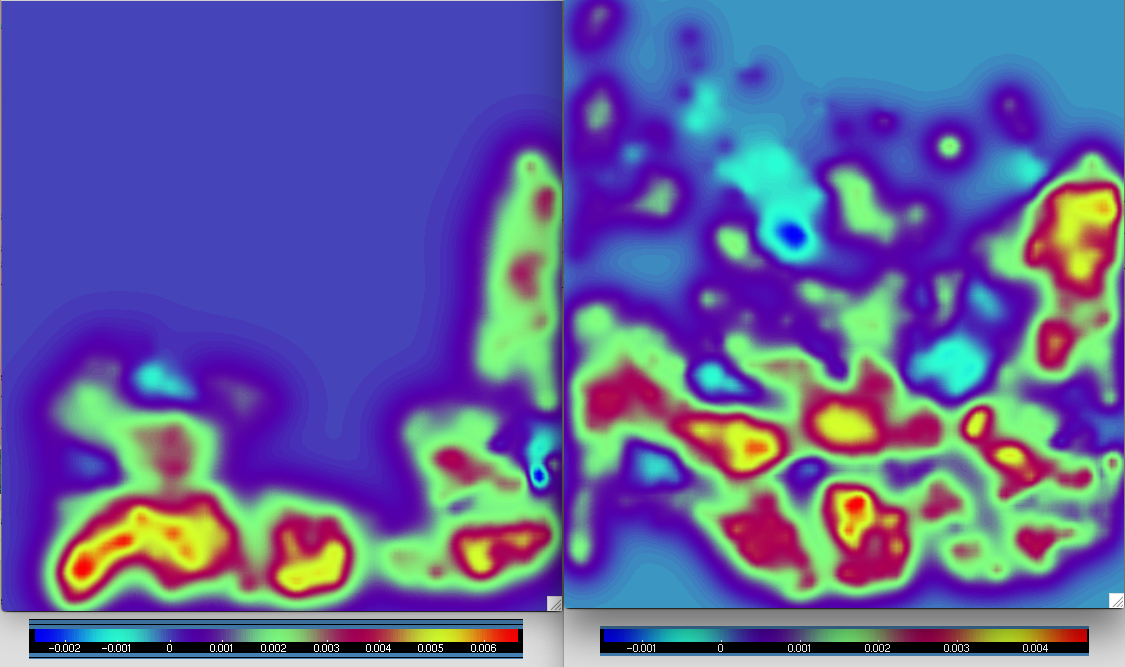
\includegraphics[width=0.8\textwidth]{./images/ch6_chem_inc_seas1_bc1.png}
  \caption{Analysis increments in the lowest level for SEAS\_1 (left) and BC1 (right).}
  \label{fig:chem}
\end{figure}

\end{enumerate}
